\documentclass{article}
\usepackage{fontspec}
\pagestyle{empty}
\usepackage{geometry}
\geometry{paperwidth=30mm, paperheight=30mm, left=2mm, top=0mm, right=2mm, bottom=0mm}
\parindent=0pt
\usepackage{color}
\usepackage{xcolor}
\usepackage{tikz}

\begin{document}
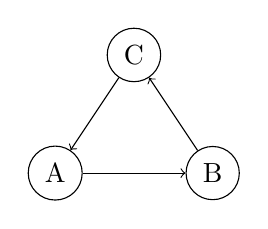
\begin{tikzpicture}
    % Define nodes
    \node[draw, circle] (A) at (0,0) {A};
    \node[draw, circle] (B) at (2,0) {B};
    \node[draw, circle] (C) at (1,1.5) {C};

    % Draw edges
    \draw[->] (A) -- (B); % Arrow from A to B
    \draw[->] (B) -- (C); % Arrow from B to C
    \draw[->] (C) -- (A); % Arrow from C to A
\end{tikzpicture}

\end{document}